\chapter{Svolgimento dello stage}
  \section{Metodo di lavoro}
    Per tutta la durata dello stage sono stati seguiti i principi del modello \textit{Agile}, usato dall'azienda per lo sviluppo dei prodotti e la gestione dei progetti.
  \section{Attività preliminari}
    \subsection{Preparazione dell'ambiente di lavoro}
      \subsubsection{Sistema operativo}
        Il primo passo e stato l'installazione e configurazione di tutti gli strumenti necessari allo sviluppo del progetto.\\
        Come sistema operativo è stato scelto Linux Mint 18.2 denominato Sonya nella versione Cinnamon, noto ambiente grafico.\\
        Si basa su Ubuntu 16.04, un versione LTS, che quindi non richiede cambiamenti ai pacchetti fondamentali.
        \begin{figure}[h]
          \centering
          
\includegraphics[scale=0.1]{immagini/linuxmint.png}
          \caption{Logo Linux Mint}
          \label{logoMint}
        \end{figure}
      \subsubsection{IDE}
        Sono stati scelti due \nameref{IDE}: IntelliJ IDEA e Android Studio.\\\\
        IntelliJ IDEA è il punto di riferimento per quanto riguarda lo sviluppo in Java, in quanto permette di utilizzare molti automatismi che semplificano la codifica, come ad esempio un autocompletamento efficace, un debugger intuitivo e semplice da usare e che agevola il controllo del programma.\\\\
        Android Studio è invece l'\nameref{IDE} ufficiale per quanto riguarda la programmazione Android.\\\\
        Si basa sul \textit{software} di IntelliJ IDEA e quindi possiede tutte le sue caratteristiche, con l'aggiunta di altri strumenti che facilitano la programmazione in Android. Un esempio è l'emulatore virtuale che permette di eseguire l'applicazione sulla stessa macchina in cui è stato scritto, oppure la possibilità di caricare l'applicazione tramite USB direttamente nello smartphone.
        \begin{figure}[h]
          \centering
          
\includegraphics[scale=0.3]{immagini/ide.png}
          \caption{Logo IntelliJ IDEA e Android Studio}
          \label{logoIntellij}
        \end{figure}
      \subsubsection{Git}
      Per quanto riguarda il versionamento del codice, è stato utilizzato Git sfruttando l'\textit{hosting} offerto da Bitbucket, dove era presente il codice sorgente delle componenti già sviluppate dall'azienda.\\
      Si è optato di avvalersi di GitKraken, un \textit{software} che permette di eseguire le operazioni classiche di Git tramite un'interfaccia grafica.
      \begin{figure}[h]
        \centering
        
\includegraphics[scale=0.5]{immagini/gitkraken.png}
        \caption{Logo GitKraken}
        \label{logoKraken}
      \end{figure}
    \newpage
    \subsection{Formazione sulle componenti esistenti}
    Dopo aver predisposto l'ambiente di lavoro è cominciata la formazione sulle componenti già esistenti, che constano dell'applicazione Android e del server Java.\\\\
    L'applicazione Android, in sostanza, è costituita da una chat che dà la possibilità di effettuare lo \textit{streaming} audio e video, con un contatto presente nella rubrica dell'applicazione.\\
    Le sue varie funzionalità sono state spiegate da uno degli sviluppatori dell'applicazione, seguendo il codice sorgente per rendere più chiaro il perché delle scelte fatte.\\\\
    Per quanto riguarda il server Java l'azienda ha fornito il codice sorgente e la documentazione.
    \subsection{Studio individuale}
      \subsubsection{Applicazione Android}
        Dopo una rapida visione del codice con lo sviluppatore dell'applicazione, lo studio individuale è continuato ripercorrendo il codice sorgente e visionando la documentazione ufficiale di Android che, essendo ben scritta e molto chiara, ha contribuito ad una maggiore comprensione delle scelte.
      \subsubsection{Server Java}
        A causa del codice non molto commentato e della documentazione troppo caotica, il funzionamento del server Java non risultava molto chiaro; l'obiettivo è stato quello di migliorarlo.
      \newpage
      \subsubsection{Eclipse Vert.x}
        \begin{figure}[h]
          \centering
          
\includegraphics[scale=0.1]{immagini/Vertx.png}
          \caption{Logo Vert.x}
          \label{logoVertx}
        \end{figure}
        La ricerca di una soluzione per il server Java necessitava di un'alternativa che permettesse uno sviluppo più semplice, che però portasse anche a un miglioramento prestazionale.\\
        Alla fine la scelta è ricaduta su Eclipse Vert.x, un \nameref{Tool} per creare ed eseguire \nameref{RA} su una \nameref{JVM}.\\
        I punti di forza osservati durante lo studio sono:
        \begin{itemize}
          \item l'alta scalabilità: è basato su eventi e non è bloccante, consente infatti di gestire molta concorrenza utilizzando pochi thread;
          \item il fatto di essere poliglotta: si può usare questo \nameref{Tool} con vari linguaggi (Java, \nameref{JS}, \nameref{Groovy}, \nameref{Ruby}, \nameref{Scala}), infatti possiede delle \nameref{API} che in automatico permettono di utilizzare il linguaggio scelto andando a lavorare comunque su una \nameref{JVM};
          \item l'ottima documentazione: è presente infatti la spiegazione di tutti i metodi nei linguaggi citati precedentemente e sono presenti anche degli esempi di codice commentati e comprensibili.
        \end{itemize}
        All'interno di questo \nameref{Tool} sono presenti numerosi moduli che permettono di eseguire azioni che, utilizzando Java nativamente, risulterebbero più laboriose e quindi più predisposte ad errori.\\
        Per utilizzare il modulo che più ci interessa, basterà configurarlo correttamente per poterlo sfruttare da subito in semplicità.\\\\
        La caratteristica principale di questo \nameref{Tool} è l'Event Loop, il thread principale che permette di richiamare i gestori degli eventi appena questi arrivano.\\
        La regola fondamentale è non bloccare mai questo loop con costrutti come wait, sleep o attese di acquisizione di lock.\\
        La scalabilità viene gestita in automatico su un'architettura multi core: nel caso arrivassero troppe richieste ad un Event Loop, ne verrebbe istanziato uno aggiuntivo su un altro core e, automaticamente, le richieste in eccesso passerebbero al nuovo Event Loop istanziato.\\
        Un altro costrutto fondamentale è l'Event Bus che permette alle diverse parti di un'applicazione di comunicare tra loro, indipendentemente dal linguaggio in cui sono scritte.\\\\
        Vert.x, inoltre, fornisce un modello di implementazione e di concorrenza semplice e scalabile. Questo modello si chiama Verticle, fornisce metodi che in automatico utilizzano l'Event loop e comunicano tra loro tramite l'Event Bus.\\
        Queste funzionalità permettono di eseguire, in modo del tutto trasparente, tutti gli automatismi del \nameref{Tool} rendendo l'applicazione molto più reattiva.
        \begin{figure}[h]
          \centering
          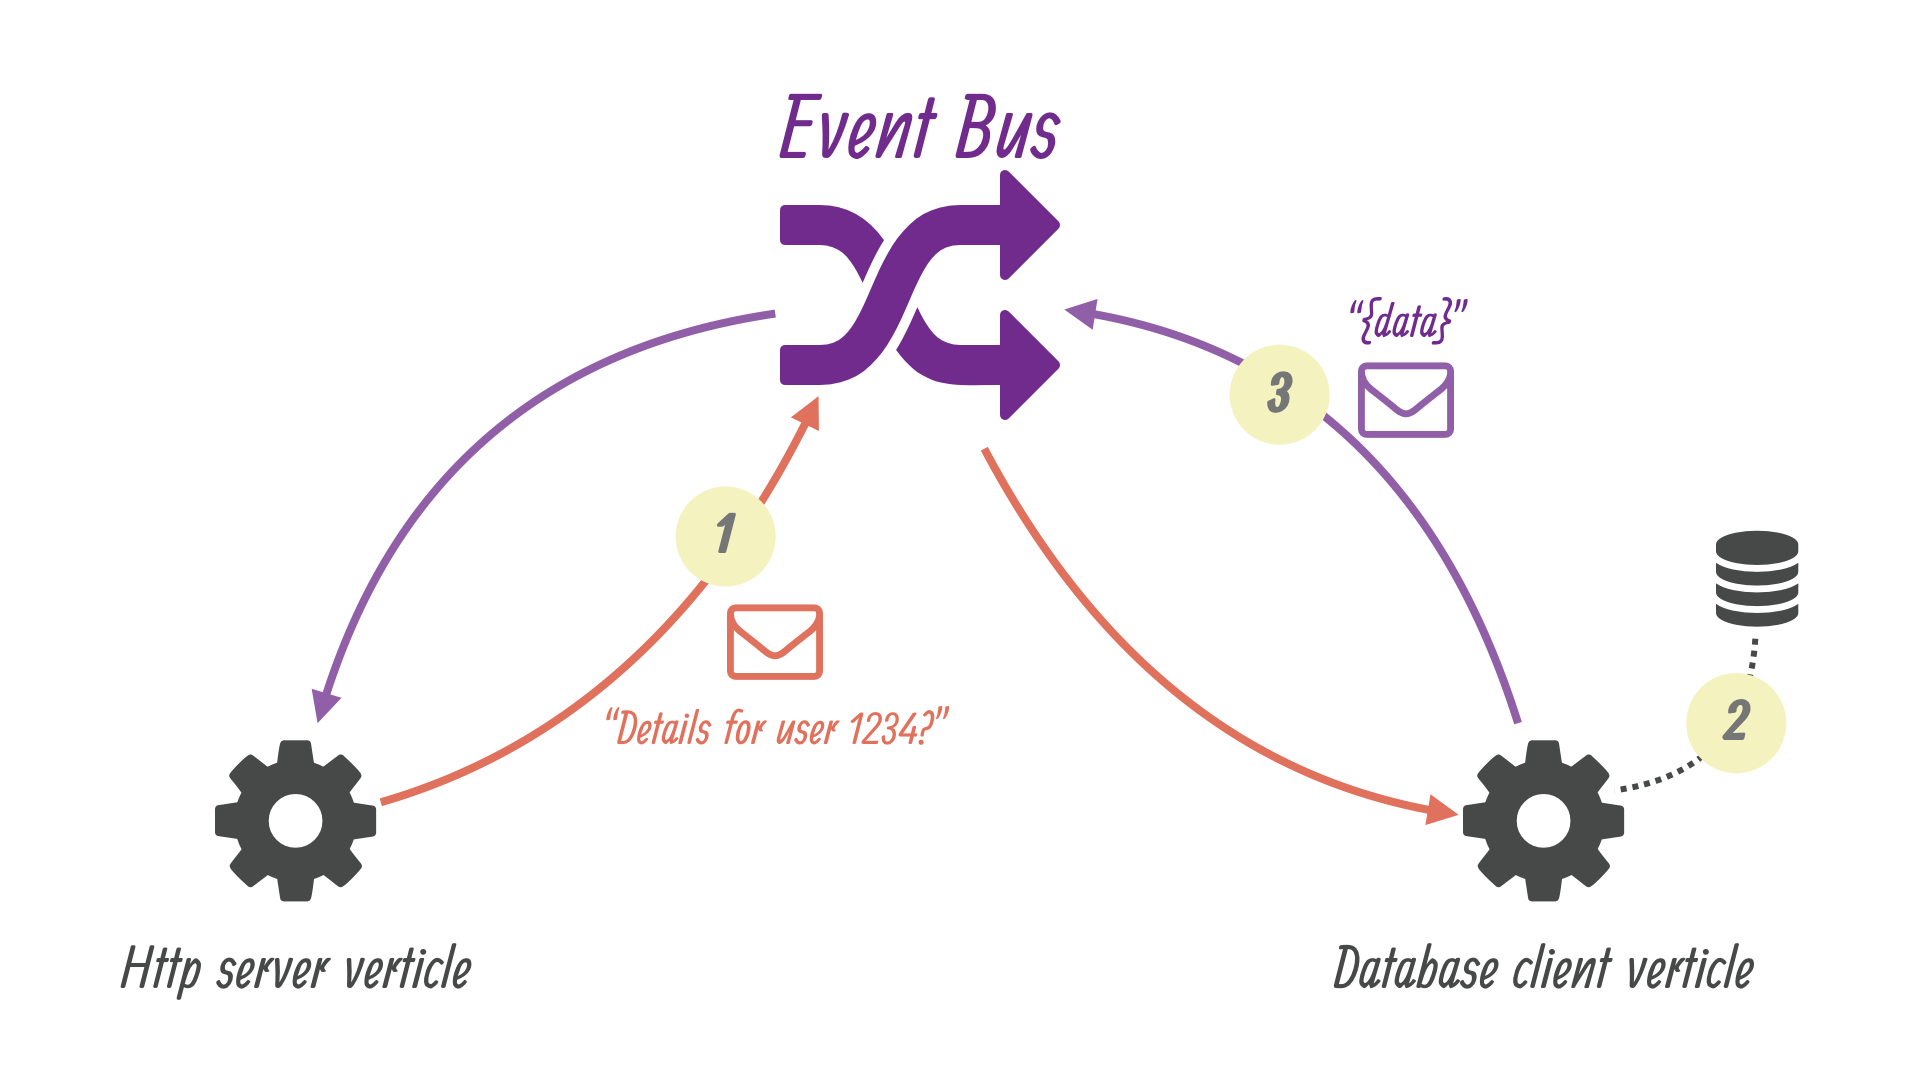
\includegraphics[scale=0.2]{immagini/event-bus.png}
          \caption{Esempio di utilizzo di due Verticle che comunicano tramite Event Bus per gestire una chiamata a database}
          \label{}
        \end{figure}
  \newpage
  \section{Sviluppo delle componenti}
    \subsection{Analisi dei requisiti}
      Le problematiche principali sono state riscontrate nel server Java quindi, in accordo con il tutor aziendale, è stato deciso di reimplementare questa componente utilizzando Vert.x.\\\\
      Lo scopo principale di questa componente è di permettere ad un utente con privilegi superiori di gestire un canale di comunicazione con uno o più utenti.\\
      In particolare deve essere possibile creare questo canale per permettere la comunicazione tra due tipi di utenti.\\
      Quindi, per ovvi motivi, deve consentire l'invio e la ricezione di messaggi e per questi deve essere possibile risalire a mittente e destinatario.\\\\
      C'è poi la necessità di discriminare tra le due tipologie di utenti che, avendo ruoli diversi, hanno anche funzionalità diverse.\\
      Deve essere presente un utente amministratore che può creare il canale di comunicazione, inviare messaggi, ricevere messaggi, limitare l'accesso ad alcuni utenti e infine chiudere il canale.\\
      Le modalità di accesso devono essere selettive, in modo da permettere all'amministratore un maggior controllo al fine di ridurre il carico di lavoro.\\\\
      L'altra tipologia di utente è quella base, cioè quella che può richiedere accesso ad un canale, inviare e ricevere messaggi nello stesso e infine abbandonarlo.\\\\
      Per ridurre l'astrazione il \textit{team} ha progettato, in parallelo, un'interfaccia grafica ed è stato richiesto, in modo facoltativo, di introdurla nell'architettura.\\
      In questo modo è possibile osservare i risultati effettivi delle funzionalità sviluppate.\\
      Un altro obiettivo opzionale è quello di integrare il sistema nell'applicazione Android, permettendo così l'effettiva unione dei due in un sistema più complesso e completo.\\
      Date le necessità descritte, si ottiene il seguente elenco dei requisiti:
      \begin{itemize}
        \item Obbligatori:
          \begin{itemize}
            \item implementazione di funzionalità che permettano di creare e gestire un canale di comunicazione;
            \item implementazione delle due tipologie di utenti distinguendo le modalità di uso del canale di comunicazione;
            \item implementazione di un sistema di permessi che permetta l'accesso solo ad utenti autorizzati.
          \end{itemize}
        \item Opzionali:
          \begin{itemize}
            \item integrazione dell'interfaccia grafica sviluppata dal \textit{team} all'interno del sistema, al fine di ridurre l'astrazione;
            \item integrazione della componente server con l'applicazione Android, in modo da creare un sistema più completo.
          \end{itemize}
      \end{itemize}
    \subsection{Progettazione}
      \subsubsection*{Canale di comunicazione}
        Nella versione precedente, il canale di comunicazione risultava di difficile comprensione e utilizzo in quanto eseguiva delle azioni considerate inutili.\\
        Si è deciso quindi di ridefinirlo e renderlo più semplice, sia di comprensione che di utilizzo.\\
        Un canale di comunicazione deve fare in modo di collegare due o più utenti, quindi in primo luogo deve essere possibile crearlo, individuarlo attraverso un identificativo e, infine, potervi accedere.\\
        Avrà quindi un identificativo che gli verrà assegnato alla creazione. È anche utile tenere una lista degli utenti che lo utilizzano in modo da semplificare poi la rimozione di uno di questi.\\
        Le funzionalità che deve offrire invece sono:
        \begin{itemize}
          \item creazione ed eliminazione;
          \item invio e ricezione di messaggi;
          \item la possibilità di rimuovere uno o più utenti dalla lista degli utilizzatori dello stesso.
        \end{itemize}
        Il concetto di messaggio viene modellato in modo molto basilare, con:
        \begin{itemize}
          \item mittente;
          \item destinatario;
          \item data e ora di invio;
          \item testo del messaggio.
        \end{itemize}
      \newpage
      \subsubsection*{Utenti}
        Un utente deve essere univoco, quindi deve avere un identificativo proprio e una password per ragioni di sicurezza, in modo da evitare usi indesiderati.\\
        Deve essere fornito di funzionalità base, quali:
        \begin{itemize}
          \item invio di messaggi attraverso il canale di comunicazione;
          \item chiusura della conversazione e dell'istanza di assistenza.
        \end{itemize}
        Ogni utente deve avere anche una tipologia, che può essere: amministratore o base. Questa distinzione è necessaria in quanto le due tipologie hanno funzioni diverse, in aggiunta a quelle di base.\\\\
        L'amministratore deve avere la possibilità di autorizzare uno o più utenti base ad accedere al canale di comunicazione.\\
        Deve anche essere possibile rimuovere una parte di utenti base che partecipano alla conversazione. Questo perché nel caso fosse stata completata l'assistenza per una parte di utenti, questi possono uscire da soli oppure devono essere rimossi, in modo da poter proseguire l'assistenza con la parte di utenti restante.\\\\
        L'utente base, invece, come funzionalità aggiuntiva presenta solo la possibilità di richiedere l'autorizzazione di accedere al canale. Questo meccanismo serve appunto a permettere all'utente base di cominciare a ricevere assistenza.
        \begin{figure}[h]
          \centering
          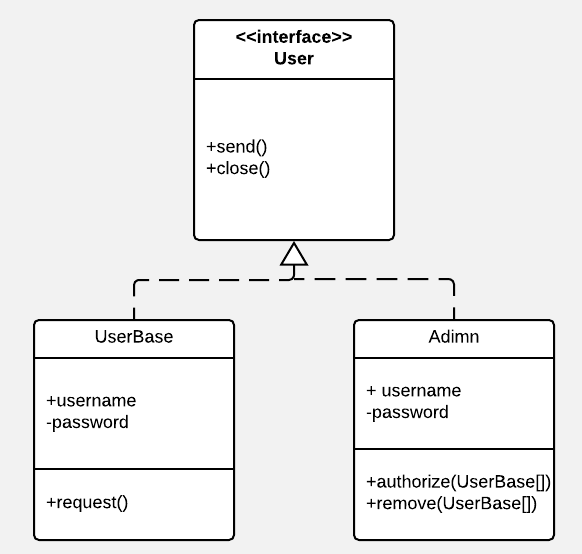
\includegraphics[scale=0.75]{immagini/user.png}
          \caption{Diagramma della classe User}
          \label{user}
        \end{figure}
      \subsubsection*{Sistema di autorizzazione}
        Deve essere possibile gestire l'accesso al canale di comunicazione. Questo verrà reso possibile sia lato amministratore sia lato utente base.\\\\
        Lato \textit{utente base} deve essere possibile effettuare una richiesta di assistenza, dalla quale segue l'autorizzazione da parte dell'amministratore. Questa richiesta viene resa possibile tramite l'invio di un messaggio contenente un testo con il tipo di assistenza che si necessita.\\\\
        Lato \textit{amministratore} deve essere possibile visualizzare le richieste effettuate dagli utenti base, l'autorizzazione a uno o più utenti ad accedere al canale di comunicazione e infine un'eventuale funzionalità di rimozione.\\
        La rimozione può essere effettuata in caso di errore oppure quando un determinato sottoinsieme di utenti non necessita di assistenza aggiuntiva.\\\\
        In questo modo è possibile gestire tutte le richieste simili in una sola volta, in modo da diminuire il carico di lavoro dell'amministratore.
      \subsubsection{Integrazione dell'interfaccia grafica}
        L'interfaccia grafica creata dal \textit{team} è composta da diverse componenti:
        \begin{itemize}
          \item struttura grafica della chat, che contiene tutte le parti di una classica chat quali:
          \begin{itemize}
            \item contenitore dei messaggi inviati;
            \item text area dove scrivere i messaggi da inviare;
            \item bottone per accedere al menù;
          \end{itemize}
          \item log in che comprende due campi dove inserire l'identificativo dell'utente e la sua password per poter accedere al sistema;
          \item menù amministratore che contiene:
          \begin{itemize}
            \item visione delle richieste;
            \item autorizzazione lista utenti;
            \item rimozione utenti dalla conversazione;
          \end{itemize}
          \item menù utente base, contenente un link a una pagina in cui è presente un form per inviare la richiesta di assistenza.
        \end{itemize}
        Entrambi i menù contengono inoltre un bottone per effettuare l'operazione di log out.\\\\
        Tutte queste componenti grafiche devono essere integrate con il sistema in modo da rendere il sistema sottostante più concreto e visibile.
        \begin{figure}[h]
          \centering
          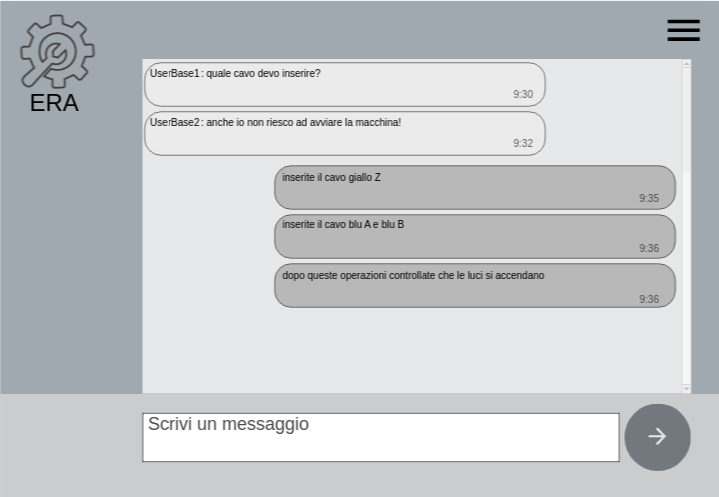
\includegraphics[scale=0.5]{immagini/chat.png}
          \caption{Esempio conversazione}
          \label{chat}
        \end{figure}
    \subsection{Implementazione}
      \subsubsection*{Canale di comunicazione}
        Come prima operazione, è stata definita la struttura JSON del messaggio.
        \begin{codice_json}[]
          {
            "sender": string,
            "receiver": string,
            "date": [
              {
                "year": number,
                "month": number,
                "day": number,
                "hours": number,
                "minutes": number
              }
            ],
            "text": string
          }
        \end{codice_json}
        \begin{description}
          \item[sender]: mittente, variabile di tipo string;
          \item[receiver]: destinatario, variabile di tipo string;
          \item[date]: data, array di variabili number contenenti anno, mese, giorno, ore, minuti;
          \item[text]: testo del messaggio, variabile di tipo string.
        \end{description}
        Successivamente come canale di comunicazione è stato scelto l'Event Bus, un oggetto fornito da Vert.x che fornisce appunto un sistema di trasmissione dati fra istanze di Vert.x.\\
        La caratteristica principale di questo bus è il fatto di essere \textit{distribuito} di default, senza la necessità di usare meccanismi come \nameref{RMI}.\\
        L'unica cosa che viene richiesta è che, alla creazione dell'Event Bus, questo venga configurato. Segue del codice di esempio.
        \begin{codice_java}
          VertxOptions options = new VertxOptions()
            .setEventBusOptions(new EventBusOptions()
            .setClusterPublicHost("IDcanale")
            ); /*tramite questo codice viene fornito l'identificativo al canale che potra' quindi essere riconosciuto anche esternamente*/
            Vertx.clusteredVertx(options, res -> {
              if (res.succeeded()) {
                Vertx vertx = res.result();
                EventBus eventBus = vertx.eventBus(); //in questo momento viene creato effettivamente l'EventBus con le impostazioni scritte precedentemente
                System.out.println("Success:" + eventBus);
              }
              else {
                System.out.println("Failed:" + res.cause());
              }
            });
        \end{codice_java}
        Le funzionalità esposte dal tipo Channel, che utilizza l'EventBus, sono state implementate utilizzando alcuni metodi propri di EventBus.
        \begin{itemize}
          \item\textbf{create(UserBase[] list):} crea l'EventBus configurandolo e aggiungendo l'amministratore e una lista di utenti base;
          \item\textbf{send(JsonObject message):} utilizza il metodo \verb+send(String address, Object message)+ di EventBus per inviare il messaggio;
          \item\textbf{remove(UserBase[] list)}: utilizza il metodo \verb+removeInterceptor(Handler<SendContext>+\linebreak \verb+interceptor)+ per rimuovere utenti base dal canale di comunicazione;
          \item\textbf{authorize(UserBase[] list)}: utilizza il metodo \verb+addInterceptor(Handler<SendContext> +\linebreak \verb+ interceptor)+ per aggiungere utenti base al canale di comunicazione;
          \item\textbf{destroy()}: utilizza \verb+close(Handler<AsyncResult<Void>> completionHandler)+ per chiudere il canale di comunicazione e rilasciare le risorse.
        \end{itemize}
      \subsubsection*{Utenti}
        Dovendo modellare due tipologie di utenti che condividono delle azioni, è stata creata un'interafaccia, User, contenente le funzionalità comuni di invio del messaggio e chiusura della conversazione.\\
        Successivamente sono state modellate altre due classi che implementano User, per creare l'amministratore, Admin, e l'utente base, UserBase.\\\\
        UserBase, oltre a implementare i metodi ereditati da User, ha anche un altro metodo che permette di effettuare la richiesta di assistenza, inviando un messaggio inserito in un \nameref{JSON}, all'amministratore.\\\\
        Admin alla stessa maniera, implementa i metodi ereditati da User, ma aggiunge due ulteriori metodi: uno che permette di autorizzare un insieme di UserBase e uno che permette la rimozione di un utente dalla conversazione.\\
        \begin{codice_java}
          public interface User{
            public void send(JsonObject);
            public void close();
          }
          public class UserBase implements User{
            public String username;
            private String password;
            public void request(){
              //corpo del metodo
            }
            //ridefinizioni dei metodi di User
          }
          public class Admin implements User{
            public String username;
            private String password;
            public void authorize(UserBase[]){
              //corpo del metodo
            }
            public void remove(UserBase[]){
              //corpo del metodo
            }
            //ridefinizioni dei metodi di User
          }
        \end{codice_java}
        Tutti questi metodi sono delle chiamate a metodo di Channel.

      \newpage
      \subsubsection*{Sistema di autorizzazione}
        Per gestire il sistema di autorizzazione è stato usato l'automatismo di default fornito da Vert.x.\\
        UserBase utilizza il metodo \verb+request()+ ed invia un primo messaggio, contenuto in un \nameref{JSON}, per indicare la richiesta di assistenza.\\
        Questo notifica ad Admin la volontà di un UserBase di ricevere assistenza.\\
        Quando arriva questa richiesta l'Admin può confermarla inserendo l'utente richiedente con l'apposito metodo \verb+authorize(UserBase[])+ nel canale di comunicazione.\\
        Il metodo, se viene chiamato per la prima volta, utilizza il metodo \verb+create(UserBase[] list)+ di Channel inserendo l'Admin e la lista di UserBase che è stata passata come argomento.\\

      \subsubsection*{Integrazione interfaccia grafica}
        Per integrare l'interfaccia grafica, fornita dal \textit{team}, scritta in \nameref{HTML}, \nameref{CSS} e \nameref{JS}, sono stati creati due Verticle, che permettono inoltre di gestire le varie componenti appena definite.\\\\
        Lato server è stato creato un Verticle, modello consigliato nell'utilizzo di Vert.x, per avviare un server \nameref{HTTP} e un server \nameref{Web}.\\
        Vert.x ha reso tutto questo molto semplice in quanto per creare il server \nameref{HTTP} è bastata una semplice chiamata a metodo:\\\\
        \verb|VertX.createHttpServer().requestHandler(httpRouteMatcher).listen(8080,"localhost");|\\\\
        Per quanto riguarda invece il server \nameref{Web}, deve inizialmente rifiutare tutte le connessioni che non possiedono l'autorizzazione per accedere al canale di comunicazione.\\
        In caso si possegga tale autorizzazione sarà possibile accedere alla conversazione.\\
        Questa si identifica nell'EventBus che permetterà, tramite l'utilizzo dei metodi citati precedentemente, la comunicazione tra amministratore e utente base.\\\\
        \newpage
        Lato \textit{client} invece è stata inserita l'interfaccia grafica fornita dal \textit{team}, aggiungendo delle funzioni \nameref{JS} per permettere le funzionalità in base al tipo di utente.\\
        Questa implementazione gestisce l'invio dei messaggi attraverso l'EventBus, la chiusura della chat e l'autorizzazione da parte dell'amministratore di utenti.\\
        Segue l'esempio del codice che permette l'invio di un messaggio.\\
        \begin{figure}[h]
          \centering
          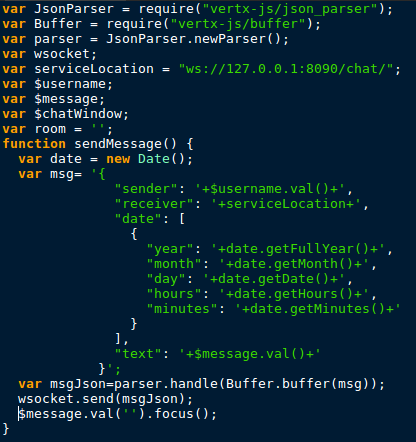
\includegraphics[scale=0.5]{immagini/sendJS.png}
          \caption{Codice per l'invio di messaggi}
          \label{cod}
        \end{figure}
  \newpage
  \section{Qualifica}
    \subsection{Verifica}
      La verifica di un prodotto è l'insieme delle operazioni che garantiscono la qualità e il rispetto delle specifiche.
      \subsubsection{Analisi statica}
        L'analisi statica consiste di \textit{test} che vengono eseguiti sul prodotto senza compilare ed eseguire codice.\\
        Questo tipo di analisi è stata delegata all'\nameref{IDE} utilizzato, in quanto fornisce strumenti di controllo di sintassi e suggerimenti sul completamento automatico.
      \subsubsection{Analisi dinamica}
        L'analisi dinamica è l'insieme delle operazioni di controllo che vengono fatte sul codice compilato ed eseguito.\\
        Per creare i \textit{test} è stato usato il modulo di Vert.x che permette di eseguirli in modo asincrono. Questo modulo utilizza delle componenti di framework come JUnit.
        Successivamente sono stati eseguiti in modo automatico, creando una \textit{pipeline} su Bitbucket.
      \subsubsection{Test}
        Vert.x permette, con il suo modulo, di creare test di unità e unirli per andare a generare una suite di test.\\
        Sono stati quindi definiti test di unità per tutte le singole componenti del sistema.\\
        Questi sono stati successivamente uniti per formare i test di integrazione che testassero il corretto funzionamento delle comunicazioni.
    \subsection{Validazione}
      La validazione di un prodotto consiste nel controllare che tutti i requisiti vengano effettivamente soddisfatti.
      \subsubsection{Validazione interna}
        Dato che il prodotto è ancora in via di sviluppo e destinato ad essere una componente di una piattaforma più grande, la sua validazione è stata interna.\\
        Sono stati eseguiti nuovamente tutti i \textit{test} e le simulazioni; infine come prova finale il tutor aziendale e un altro componente del \textit{team} hanno provato a comunicare tra di loro utilizzando il prodotto.
  \section{Analisi dei principali problemi}
    \subsection{Utilizzo Vert.x}
      Essendo tutto il progetto basato sull'utilizzo di Vert.x, lo studio di questo \nameref{Tool} ha portato a dei problemi.\\
      Questo perché presenta un insieme molto grande di moduli e quindi ha richiesto una mole di studio per comprendere appieno quali effettivamente bisognava usare.\\
      Tuttavia, seguendo la documentazione e visionando numerosi esempi, è stato possibile  restringere il campo d'azione e trovare e poi utilizzare i moduli che risultavano più corretti.
    \subsection{Metodo Agile}
      Inizialmente seguire il metodo \textit{Agile} è stato difficile, in quanto il tutor era spesso fuori sede o comunque concentrato su altri progetti.\\
      Tuttavia era comunque presente su i canali di comunicazione e rispondeva in tempi brevi.\\
      Una migliore pianificazione probabilmente avrebbe permesso di proseguire in modo più fluente il lavoro.
      \newpage
      \null
      \thispagestyle{empty}
